\paragraph{Задание 2}

\begin{gather*}
    \bar{x_{s}} - t\frac{s}{\sqrt{n}} < \bar{x_{tr}} < \bar{x_{s}} + t\frac{s}{\sqrt{n}}\\
    t_{0.025;159} = 1.975\\
    \bar{x_{s}} \in (433.1038; 481.6509)
\end{gather*}

\begin{gather*}
    s \cdot q_{1} < \delta_{tr} < s \cdot q_{2}\\
    q_{1} = \sqrt{\frac{n - 1}{\chi_{0.025;159}}}\\
    q_{2} = \sqrt{\frac{n - 1}{\chi_{0.975;159}}}\\
    \delta_{tr} \in (142.0230; 170.7810)
\end{gather*}

\begin{gather*}
    p_{i} = P(x_{i-1} < X < x{i}) = \Phi(\frac{x_{i} - \bar{x}}{\delta}) - \Phi(\frac{x_{i - 1} - \bar{x}}{\delta})
\end{gather*}

\begin{table}[H]
    \begin{center}
        \begin{tabular}{|l|l|l|l|}
            \hline
            \multicolumn{2}{|c|}{$[x_{i}..x_{i+1}]$} & Частоты $n_{i}$ & Выравнивающие частоты $n{}' = np_{i}$ \\
            \hline
            9       & 58.889  & 1  & 0.505  \\
            \hline
            58.889  & 108.778 & 2  & 1.149  \\
            \hline
            108.778 & 158.667 & 2  & 2.355  \\
            \hline
            158.667 & 208.556 & 4  & 4.356  \\
            \hline
            208.556 & 258.445 & 10 & 7.272  \\
            \hline
            258.445 & 308.334 & 7  & 10.954 \\
            \hline
            308.334 & 358.223 & 13 & 14.889 \\
            \hline
            358.223 & 408.112 & 20 & 18.261 \\
            \hline
            408.112 & 458.001 & 17 & 20.211 \\
            \hline
            458.001 & 507.890 & 23 & 20.185 \\
            \hline
            507.890 & 557.779 & 22 & 18.191 \\
            \hline
            557.779 & 607.668 & 13 & 14.793 \\
            \hline
            607.668 & 657.557 & 10 & 10.856 \\
            \hline
            657.557 & 707.446 & 10 & 7.188  \\
            \hline
            707.446 & 757.335 & 2  & 4.295  \\
            \hline
            757.335 & 807.224 & 2  & 2.316  \\
            \hline
            807.224 & 857.113 & 1  & 1.127  \\
            \hline
            857.113 & 907.002 & 1  & 0.495  \\
            \hline
        \end{tabular}
    \end{center}
\end{table}

\begin{table}[H]
    \begin{center}
        \begin{tabular}{|l|l|l|}
            \hline
            Частоты $n_{i}$ & Выравнивающие частоты $n{}' = np_{i}$ & $(n{}'_{i} - n_{i}) / n{}'_{i}$ \\
            \hline
            5               & 4.009                                 & 0.245                           \\
            \hline
            4               & 4.356                                 & 0.029                           \\
            \hline
            10              & 7.272                                 & 1.024                           \\
            \hline
            7               & 10.954                                & 1.427                           \\
            \hline
            13              & 14.889                                & 0.240                           \\
            \hline
            20              & 18.261                                & 0.166                           \\
            \hline
            17              & 20.211                                & 0.510                           \\
            \hline
            23              & 20.185                                & 0.392                           \\
            \hline
            22              & 18.191                                & 0.797                           \\
            \hline
            13              & 14.793                                & 0.217                           \\
            \hline
            10              & 10.856                                & 0.067                           \\
            \hline
            10              & 7.188                                 & 1.100                           \\
            \hline
            6               & 8.232                                 & 0.605                           \\
            \hline
        \end{tabular}
    \end{center}
\end{table}

$\chi^2_{watch} = \sum_{}^{} (n{}'_{i} - n_{i}) / n{}'_{i} = 6.8199$ Для уровня значимости $\alpha = 0.05$ и $k = 10$ соответствует значение $\chi^2_{crit} = 18.3070$.
Так как:
\[\chi^2_{watch} < \chi^2_{crit} \]

\begin{table}[H]
    \begin{center}
        \begin{tabular}{|l|p{0.25\linewidth}|p{0.25\linewidth}|l|}
            \hline
            Частоты & Эмпирическая функция распределения $F{}'(x)$ & Теоретическая функция распределения $F(x)$
            & Разности $\left| F{}'(x) - F(x) \right|$
            \\
            \hline
            1  & 0.006 & 0.005 & 0.001 \\
            \hline
            2  & 0.019 & 0.012 & 0.007 \\
            \hline
            2  & 0.031 & 0.027 & 0.004 \\
            \hline
            4  & 0.056 & 0.054 & 0.002 \\
            \hline
            10 & 0.119 & 0.100 & 0.019 \\
            \hline
            7  & 0.162 & 0.168 & 0.006 \\
            \hline
            13 & 0.244 & 0.261 & 0.017 \\
            \hline
            20 & 0.369 & 0.375 & 0.007 \\
            \hline
            17 & 0.475 & 0.502 & 0.027 \\
            \hline
            23 & 0.619 & 0.628 & 0.009 \\
            \hline
            22 & 0.756 & 0.741 & 0.015 \\
            \hline
            13 & 0.837 & 0.834 & 0.004 \\
            \hline
            10 & 0.900 & 0.902 & 0.002 \\
            \hline
            10 & 0.962 & 0.947 & 0.016 \\
            \hline
            2  & 0.975 & 0.974 & 0.001 \\
            \hline
            2  & 0.987 & 0.988 & 0.001 \\
            \hline
            1  & 0.994 & 0.995 & 0.001 \\
            \hline
            1  & 1.000 & 0.998 & 0.002 \\
            \hline
        \end{tabular}
    \end{center}
\end{table}

\begin{gather*}
    \lambda_{watch} = \sqrt{n}\cdot\max_{x}\left| F{}'(x) - F(x) \right| = 0.3365\\
    \lambda_{crit} = 1.36\\
    \lambda_{watch} < \lambda_{crit}
\end{gather*}

Нет оснований отвергать гипотезу о нормальном распределении.

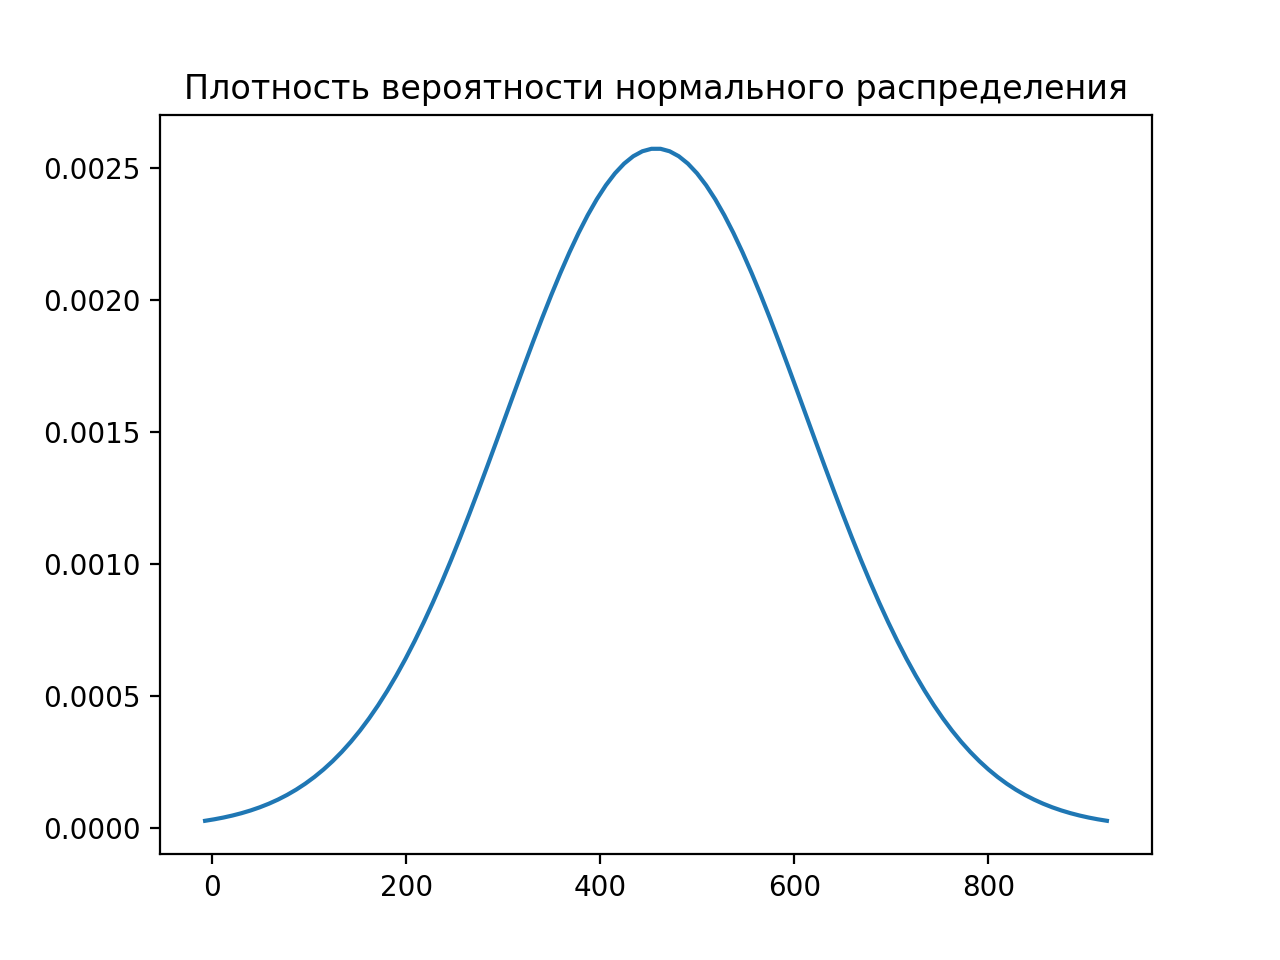
\includegraphics[width=0.9\textwidth]{src/gr21}

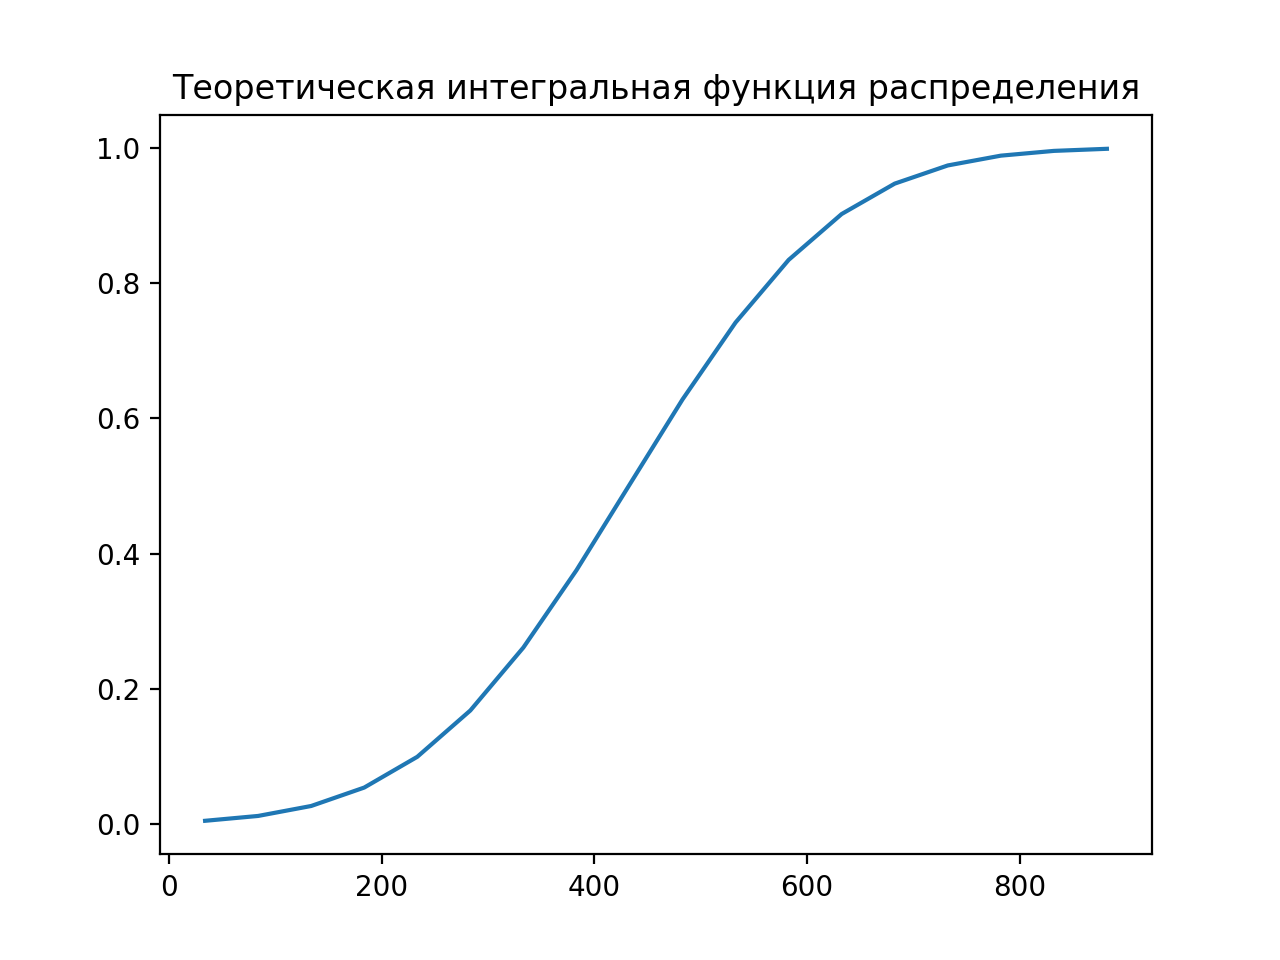
\includegraphics[width=0.9\textwidth]{src/gr22}
